\section*{Examples}
\aa{Example 1: nothing to add, I think it is great as is. Figures 3 and 4 are very informative now. Great job! 
Example 2: it is nicely exposed, although the results don't seem too promising. You said you got new, better results, so that’s good news. ;-)}

Our modelling framework is best explained with concrete examples. 
In this section we first present how experimental results could be introduced as prior knowledge of the fundamental niche in a species distribution model (\ac{SDM}), and in the following we apply our approach to integrating phenological information with occurrence data for a widespread North American tree.
\ia{delete the above paragraph}
\mt{I tend to agree}

%---------------------------------------------
\subsection*{Example 1: Adding experimental evidence for the fundamental niche to a species distribution model} 

In this hypothetical example, we build a metamodel relating the distribution (i.e. occurrence probability) of an annual plant to coarse-scale climate with complementary information originating from a fine-scale experiment manipulating the precipitation regime.
The metamodel attempts to capture the realized distribution of a species, thereby encapsulating in a single correlative model the major physiological constraints and ecological processes constraining a species distribution. 
\mjf{How does it capture these constraints if it is a correlative model?}
However, for the purposes of forecasting, we would like to disentangle the fundamental response of a species to environmental variation from other processes in order to map the climatic envelope of where a species may be found in a natural setting. 
Prior information of the physiological constraints affecting species distribution is sometimes available, but usually too incomplete to perform a reasonable comparison with the realized distribution.
For instance, as in this example, a species distribution might be constrained by both temperature and precipitation, but experiments were conducted only over a precipitation gradient at one temperature. 
\dm{May want to provide a bit more justification as to why this particular hypothetical example is useful? When I think of experimental data I think you are meaning lab-controlled data which is quite rare I think?}
We apply our framework here to such heterogeneous sources of information to reduce the bias in parameter estimation and more adequately represent uncertainty. 
Here, we focus only on the specification of the modelling framework; complete procedural details and code for generating the data sets and executing the model are provided as supplemental information.

We consider data collected from a species' historical distribution, where the goal is to predict the distribution following a substantial reduction in precipitation. 
We will consider \(X_M\) (see Box 1, Fig. \ref{fig:diagram}) to be a vector of $n$ observations that takes the value of one to indicate presence and zero for absence:
\begin{equation}
X_M = \{x_{M,1}, x_{M,2}, \ldots, x_{M,n}\}
\end{equation}
\dm{Just noting my initial comment that even absence data can be of course tricky eg structural zeros; a cryptic species; looked at the wrong time of day; some disturbance happened that year….etc….etc.  I note your comment in the next sentence which is good}
We further assume the data are relatively high-quality, providing coverage over a wide region and covering various climatic conditions (Fig. \ref{fig:ex1_sampling}a). 
The model is evaluated by relating these observations to environmental data \((D_M)\), which for the sake of the example consists of mean annual temperature $T_M$ and annual precipitation $P_M$. 
For simplicity, we use a simple logistic model for the metamodel \((\theta_M)\) with a second order effect of temperature and precipitation. 
This naive model (i.e., the metamodel with no constraints from sub-models) predicts  occurrence probability (\(\psi_N\)) as a function of the environment:
%-----
\begin{equation}
\begin{aligned}
	\psi_N &= f\left(\theta_M, D_M \right) \\
	&= p \left (X_M = 1 \mid \theta_M, T_M, P_M \right) \\
	&=\text{logit}^{-1}\left( \mathbf{\Theta_M} \mathbf{D_M} \right)
\end{aligned}
\end{equation}
%-----
where \(\mathbf{\Theta_M}\) is the parameter vector of the model \(\theta_M\), \(\mathbf{D_M} \) is the covariate matrix (i.e., \(T_M, P_M\), with the first column taken to be unity to allow an intercept to be fit), and \(\text{logit}^{-1}\) is the inverse of the logit function.
We can fit this model in a Bayesian framework to allow for easy integration of models (as we will show later).
In this context, the goal of modelling is to estimate the probability distribution of \(\theta_M\), the model parameters, given the observed data \((X_M, T_M, P_M)\), which is given by the proportional form of Bayes's Theorem \citep[for readers unfamiliar with general concepts in Bayesian inference, we recommend][for a concise introduction]{Link2010}:
\fd{Bonne idée d'avoir introduit cette proposition ici.}
\dm{add citation: McCarthy M.A. 2007 Bayesian methods for Ecology. Cambridge University Press 296p}
\dm{Mick McCarthy might be a good suggestion for a reviewer (I know him – an Aussie)}
%-----
\begin{equation}
\label{eq:ex1_bayes}
	p\left (\theta_M \mid X_M,T_M,P_M \right ) \propto 
	p \left(X_M \mid \theta_M, T_M, P_M \right)
	p \left(\theta_M \right)
\end{equation}
%-----
where \(p\left(X_M \mid \theta_M, T_M, P_M \right)\) is often referred to as the \emph{likelihood} of the data (\(X_M\)) given the model (\(\theta_M\)), \(p\left(\theta_M \right)\) is often referred to as the \emph{prior distribution} of \(\theta_M\), and the goal of modelling is to estimate \(p\left (\theta_M \mid X_M,T_M,P_M \right )\), the \emph{posterior distribution} of \(\theta_M\), which gives the probability that \(\theta_M\) takes particular values, given the observed data.

%==================
% FIGURE

\begin{figure}[tb]
	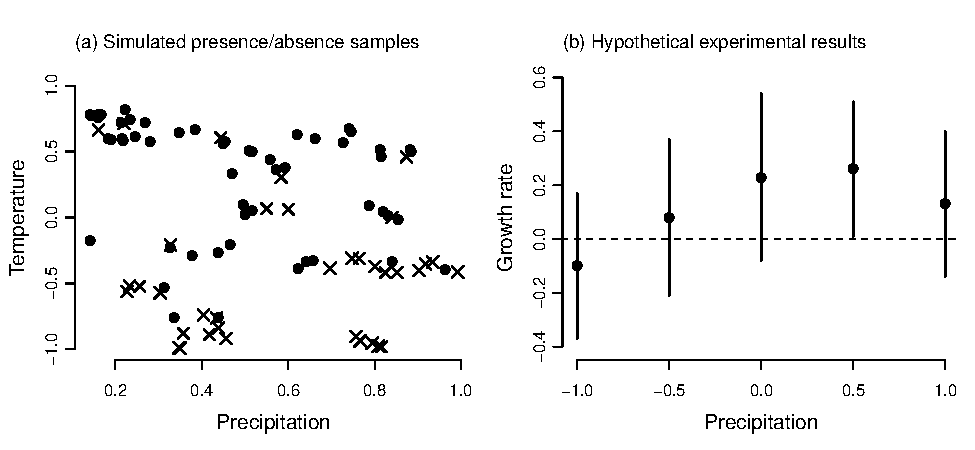
\includegraphics{ex1_sampling.pdf}
	\caption{Two simulated data sets used to illustrate the model integration framework.
	(a) Presences (circles) or absences (x's) of the species in ecological space, where precipitation ranges from 0--1.
	(b) Growth rate ($r$) as a function of manipulations to the precipitation regime (whiskers show $\pm$ 1 SE), with a larger range for precipitation (i.e., \(-\)1--1).
	The dashed line shows the threshold above which the species net growth rate is positive (implying presence).
	Axis scales for temperature and precipitation are arbitrary, but note the different scales on the horizontal axes.}
	\label{fig:ex1_sampling}
\end{figure}

% ERUGIF
%==================

Thus far, we have considered only a single source of information to fit this model, and therefore the prior distribution \(p\left(\theta_M \right)\) from Eq. \ref{eq:ex1_bayes} is uninformative.
As a secondary source of information, we will consider an experiment relating the population growth rate of the plant to manipulations to the precipitation regime, with results (but no raw data) available from the literature (Fig. \ref{fig:ex1_sampling}b). 
Furthermore, no information is available regarding the temperature regime for the experiment.
Transplant experiments that evaluate performance beyond the range of a species are common, and represent a plausible scenario for model integration \citep{Hargreaves2014}.
According to niche theory \citep{Holt2009}, the fundamental niche corresponds to the set of environmental conditions where the per capita intrinsic growth rate $r$ is positive.
This concept gives us a reasonable model to fit the scaling function $g$ for our sub-model (Fig. \ref{fig:diagram}).
If we hypothesize that the errors from Figure \ref{fig:ex1_sampling}b \( \left(\sigma_{S} \right) \) are normally distributed, then for observation $i$, we can interpret the probability of presence \( \left(\psi_{S,i}\right)\) as the probability that the observed growth rate \(X_{S,i}\) is positive:
\begin{equation}
	\psi_{S,i} = \int_0^\infty N \left(X_{S,i}, \sigma_{S,i} \right)
\end{equation}
where \(N\) is the Normal density function.
We can then estimate the posterior distribution for the sub-model by fitting the relationship between \(\psi_S\) and precipitation \( \left( P_S \right) \) using Bayesian beta regression \citep{Ferrari2004}:
%-----
\begin{equation}
\label{eq:ex1_thetas}
	p\left (\theta_S \mid \psi_S,P_S \right ) \propto 
	p \left(\psi_S \mid \theta_S, P_S \right)
	p \left(\theta_S \right) \\
\end{equation}
%-----

Although the two data sets were collected at considerably different scales, we now have sub-model predictions arising from a fine-scale experiment that are relevant at the scale of the metamodel (i.e., the probability of presence at a given precipitation). 
This scaling is quite simplistic, and would never be used to predict a species' range using this mechanistic sub-model in isolation.
Despite the strong theoretical foundation (i.e., niche theory) linking the observations to presence-absence at large scales, the upscaled sub-model (i.e., the transformation of \(X_S\) and \(\sigma_S\) to \(\psi_S\)) is built on the strong hypothesis that the species will be present when $r>0$, neglecting other population dynamics constraints such as Allee effects and metapopulation dynamics. 
The fundamental niche is also incomplete, as we lack environmental variables such as temperature, as well as all other ecological processes responsible for the realized distribution.
As such, it would be unwise to expect predictions from this model alone to resemble the actual distribution of the species; as a mechanistic model, it is simply too incomplete to predict distribution.
As we will show, however, the information from this sub-model, when applied as a constraint on the metamodel, can result in improved predictions that incorporate the information within each model.

We accomplish model integration by treating the posterior of \(\theta_S\) as prior information about some of the parameters of \(\theta_M\) (i.e., parameters related to precipitation), expanding Equation \ref{eq:ex1_bayes} to incorporate the new information from the sub-model:
%-----
\begin{equation}
	\label{eq:ex1_integrated}
	\overbrace{p(\theta_M \mid X_M, T_M, P_M, \theta_S, \psi_S, P_S)}^\text{integrated posterior}
	\propto
	\overbrace{p\left (\psi_S \mid \theta_S,P_S \right )}^{\substack{\text{new information} \\ \text{from sub-model}}}
	\overbrace{p \left(X_M \mid \theta_M, T_M, P_M \right) P \left(\theta_M \right)}^{\substack{\text{naive metamodel} \\ \text{posterior}}}
	\overbrace{p \left(\theta_S \right)}^{\substack{\text{prior for} \\ \text{sub-model}}}	
\end{equation}
%-----
As before, the metamodel \(\theta_M\) can be used to predict the species distribution \((\psi_I)\).
However, these predictions will not reflect only the presence-absence samples in \(X_M\), but will also reflect the information from \(\theta_S\), including all of the data sources used to produce this sub-model.
In other words, with this evaluation, the set of parameters $\theta_M$ is most likely when it agrees with both the original data and predictions from the sub-model. 
Note that in this particular example, because the sub-model is only contingent on precipitation, there is no integration on temperature. 
Finally, we note the presence of marginal distributions for both models (i.e., \(p(\theta_M)\) and \(p(\theta_S)\)).
These can be informative (e.g., incorporating further prior information or the predictions of additional sub-models), semi-informative (e.g., to provide greater weight to more informative models), or uninformative.
\fd{A word should be said about how the likelihood function balance the two sources of information for (Psi)M.  (How greater weight can be given to a more informative sub-model).}
For purposes of this example, we used these terms to reduce the precision of the second model to reflect the uncertainty of the modelling process (due to the lack of additional mechanisms in the second model, as mentioned above).
\fd{MAYBE NOT EXACTLY THERE:  "Moreover, convergent or divergent sub-models' response in ovelapping scale domains can  help in detecting crucial ecological processes."}

We performed this procedure with our hypothetical data sets.
When comparing the three models (naive metamodel, mechanistic sub-model, and integrated metamodel), we observed extreme uncertainty in the first model when projecting beyond the range of the original data.
Unsurprisingly given the quality of the data, the sub-model was highly precise, providing a fairly strong constraint when producing the integrated model.
The result was an integrated prediction that reflected the shapes of both models and showed considerably reduced uncertainty (Fig. \ref{fig:ex1_precip}).
At the scale of the metamodel, considering both temperature and precipitation, we observed similar results, with reduced uncertainty in the predictions over the domain not covered by the presence-absence data (Fig. \ref{fig:ex1_map}).


%==================
% FIGURE

\begin{figure}[tb]
	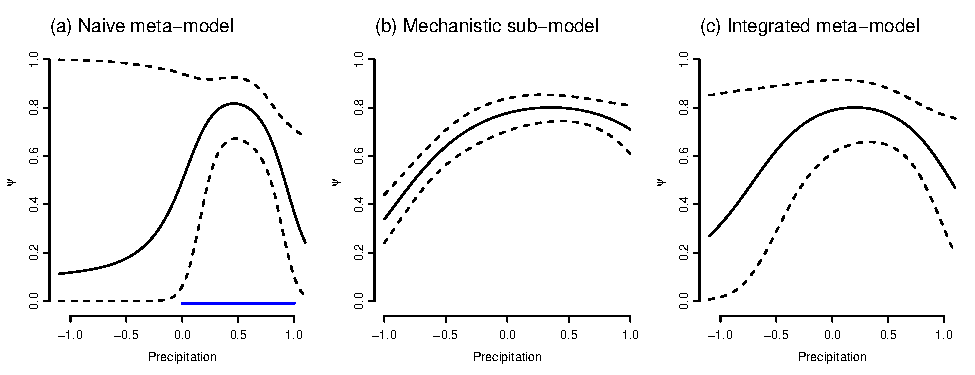
\includegraphics{ex1_precip.pdf}
	\caption{Results of integration showing the probability of presence (\(\psi\)) when considering only precipitation.
	(a) Naive model, using only presence-absence data. Uncertainty increases dramatically when attempting to project beyond the scope of the source data (represented by the horizontal line above the bottom axis).
	(b) Mechanistic model, using observations of an experiment to infer probability of presence. Predictions are highly precise due to high quality source data, but are likely to be overly optimistic given the simplicity in assuming only precipitation determines probability of presence (see text).
	(c) Integrated model, showing predictions that are intermediate between the two sub-models and uncertainty that is reduced compared to (a).
	Uncertainty is represented as dashed lines, showing the limits of 90\% Bayesian credible intervals.}
	\label{fig:ex1_precip}
\end{figure}
% ERUGIF
%==================


%==================
% FIGURE

\begin{figure}[tb]
	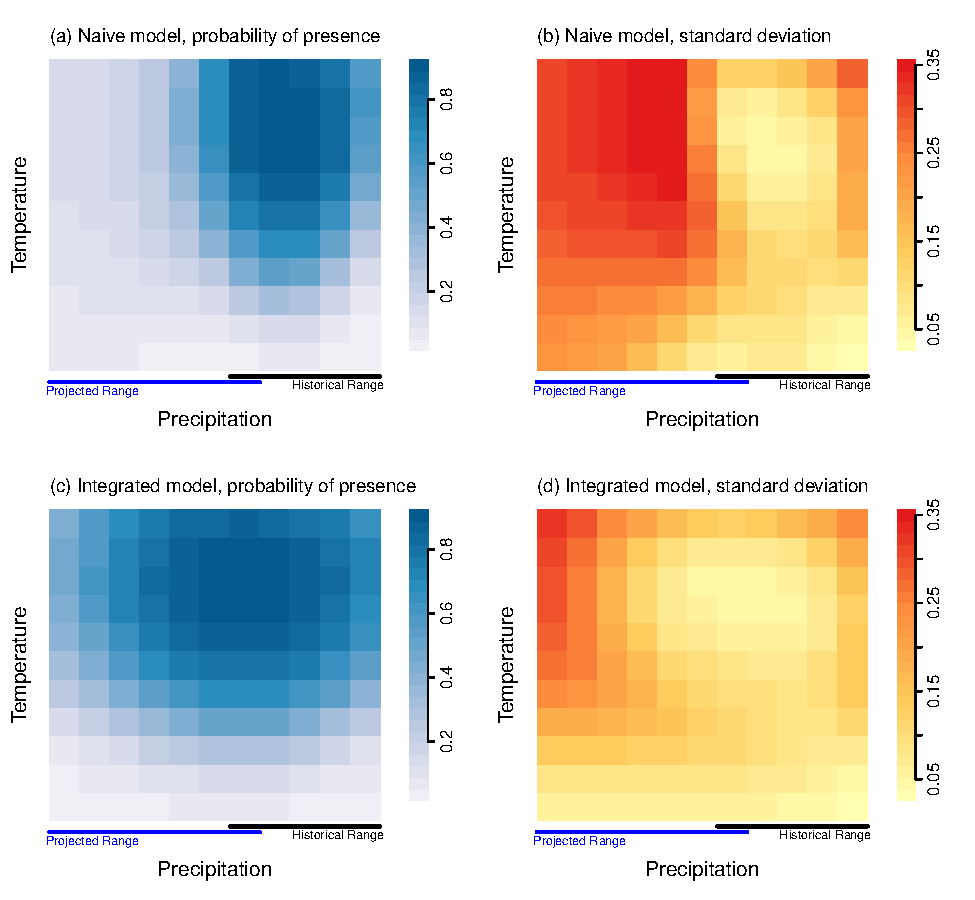
\includegraphics[width=5.25in]{ex1_map.pdf}
	\caption{Maps showing the predicted probability of presence (\(\psi\); (a) and (c)) and the standard deviation of \(\psi\) ((b) and (d)) for the naive and integrated models.
	Historical (e.g., where presence-absence samples were available) and predicted future precipitation regimes are shown below the horizontal axes.
	Uncertainty in the naive model was extreme when predicting beyond the historical precipitation regime.
	Uncertainty in the integrated model was considerably reduced, reflecting the additional information provided by the mechanistic model.}
	\label{fig:ex1_map}
\end{figure}
%
% ERUGIF
%==================
\dm{FIG 4: Again just a comment …one could discuss what does this probability of presence really mean?  Presence with a self sustaining population. Someone could plant a specimen outside its historic natural range and expect it to live.  I woder if rather than naïve the term "simple" would be better? I have substituted for that word in some places …Aren’t we all naïve ??!!}

Once the technical challenges of evaluating the parameters are overcome, the integration has several advantages over the both the naive parameterization of the metamodel and the mechanistic sub-model. 
In the situation where both models strongly agree on the relationship between water availability and occurrence probability, then we should expect significantly reduced uncertainty in that domain (Figs. \ref{fig:ex1_precip}, \ref{fig:ex1_map}).
Because the metamodel includes both temperature and precipitation, any reduction in the uncertainty with respect to precipitation might also influence the evaluation of the relationship with temperature (reducing bias in the case where there is a correlation between T and P in the data). 
However, uncertainty could increase in the case of model disagreement.
For instance, the relationship between precipitation and presence in the naive metamodel could be caused by a spurious relationship (e.g. spatial autocorrelation caused by historical contingencies), leading to a false confidence in the species distribution over precipitation gradients. 
The information from the sub-model will thus bring back the right amount of uncertainty in the relationship.

\subsection*{Example 2: Constraining an SDM using phenological information}
For the second example, we consider the problem of predicting the future distribution of a species following climate change.
There is considerable interest in comparing correlative and mechanistic projections with respect to climate change \citep{Morin2009}, and correctly characterizing uncertainty is a critical aspect of this problem \citep{Cheaib2012}.
Despite being a relatively common application of \ac{SDM}s \citep{Guisan2005}, projecting models parameterized with modern climate data to future climate scenarios is problematic for a number of reasons previously discussed \citep{Araujo2006, Austin2011}.
We used our metamodeling framework to inform a climate-based SDM with information obtained from Phenofit, a mechanistic model that predicts a species' probability of presence as a function of the suitability of the environment given the species' phenology \citep{Chuine2001, Morin2009}.
We use data from \citet{Morin2009} for sugar maple (\emph{Acer saccharum}), an economically and ecologically important species occurring in eastern North America.
Here we describe briefly the dataset, methods, and the results of the analysis.
Complete details, including all data and scripts to reproduce the analysis, are included as supplemental information.

\defcitealias{IPCC2001}{IPCC, 2001} %% this is needed to make the organizational citation in the following paragraph work correctly
For the metamodel, we used a dataset of 1013 sugar maple presence records at 0.5 degree resolution, with 498 corresponding pseudo-absence records sampled from North America.
\mt{update numbers with final versions, and indicate that they are true absences}
We used a binomial GLM to relate the suitability for sugar maple to 5 climate variables, scaled to the same resolution (see SI for a description of the climate variables used).
fd{Present the abbreviation for SI= Supplemental Information earlier in the text (at the end of the previous paragraph, for example.)}
\wt{We could also have used something more complex such as a GAM or boosted regression trees. }
\mt{Perhaps note this; we selected this model for simplicity of explanation and implementation, but more flexible functions are possible}
For projection, we used predictions for 2080 from the HadCM3 GCM \citep{Pope2000} driven by the A2 emission scenario (REF--Nakicenovic), and used the parameters of the GLM to forecast suitability into the future (i.e., \(\psi_N\)).
\wt{citation:
Nakicenovic, N. \& Swart, R. (ed.\^eds) (2000) Emissions Scenarios: A Special Report of Working Group III of the Intergovernmental Panel on Climate Change. Cambridge University Press, Cambridge.}
\tf{Is it an optimistic or pessimistic or medium scenario? 
Would it be interesting to compare two extreme scenarios? Would it change something to the demonstration of this manuscript?}
Phenofit produces predictions at continental scales; thus the scaling function \(g\) was incorporated within Phenofit itself and we performed model integration directly on the outputs.
To perform the integration, we used \ac{MCMC} to condition the parameters of the metamodel simultaneously on two likelihood functions.
The first is the naive SDM, where the likelihood of a ``success'' in the presence/pseudo-absence dataset was a Bernoulli density with the (logit-transformed) probability expressed as a linear function of the climate predictors.
The sub-model likelihood was the Beta density of the observed Phenofit prediction for the present climate given the predicted suitability under the naive model. 
Thus, the posterior probability of the metamodel was:
\begin{equation}
\label{eq:integrated2}
	p( \theta_M \mid X_M, D_M, X_S, \theta_S )
	\propto 
	p( X_S \mid \theta_M, \theta_S )
	p( Y_M \mid \theta_M, D_M ) 
	p( \theta_M )
	p( \theta_S )
\end{equation}
where \(\theta_M\) is the metamodel, 
\(X_M\) is the vector of presences and pseudo-absences, 
\(D_M\) is the matrix of climate predictors,
\(X_S\) is the prediction from Phenofit (in this case a single deterministic value, because we did not incorporate errors from the Phenofit modelling),
and \(\theta_S\) is the model relating the Phenofit predictions to the metamodel.
\fd{Shouldn't be Psi\_S here as we speak of prediction of the sub-model?}
Note that here, the integration is performed on the \emph{predictions} of the sub-model directly, rather than on compatible parameters as in Example 1. Thus, the metamodel must appear in the sub-model likelihood.

The naive model, despite being relatively simple (xx climate variables with xx total parameters), was highly fit to the data and consequently showed very high suitability scores near the core of the contemporary range with very little uncertainty (Fig \ref{fig:ex2}C, E).
Similar patterns were repeated for analogous climates under the future scenario (Fig \ref{fig:ex2}D, F).
However, standard errors were extreme for the range margins where suitability scores were intermediate.
In comparison, Phenofit suitability scores were more moderate, and Phenofit predicted less northward movement of sugar maple under the future scenario \citep[Fig. \ref{fig:ex2}A, B;][]{Morin2009}.
The integrated model demonstrated generally lower suitability scores throughout both the present and projected ranges, and thus represents lower confidence in the presence of sugar maple at any given location in its future projected range (Fig \ref{fig:ex2}G, H).
Standard errors at range margins were significantly lower (as these are regions where both the naive model and phenofit were in agreement about intermediate suitability scores), whereas standard errors were slightly higher at the core range (where Phenofit predicted lower suitability than the naive model) (Fig \ref{fig:ex2}I, J).

%==================
% FIGURE

\begin{figure}[tb]
	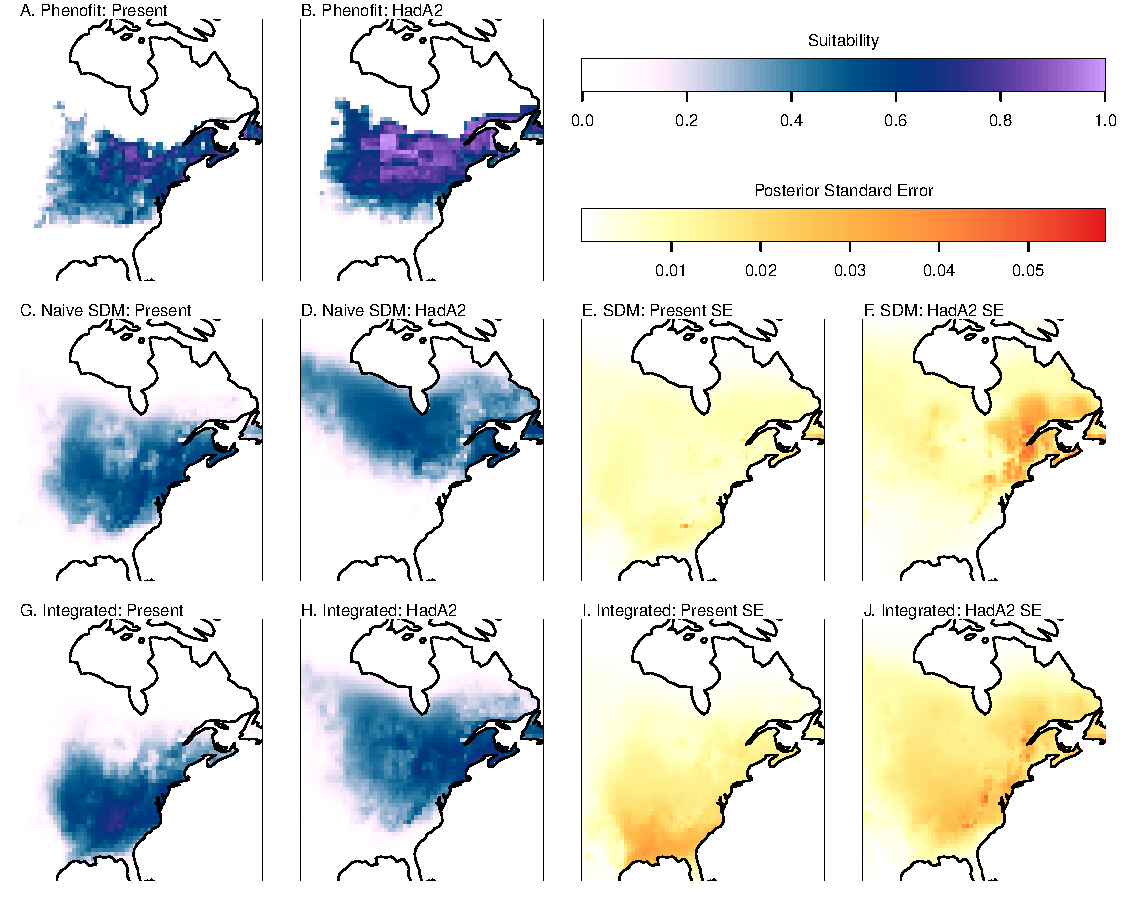
\includegraphics[width=6in]{ex2.pdf}
	\caption{Results of model integration for sugar maple, \emph{Acer saccharum}.
	The mechanistic sub-model Phenofit predicts present (A) and future (B) suitability using phenological information, but does not provide estimates of uncertainty.
	Predictions from a naive metal-model for the present (C) were quite similar to the sub-model, but future predictions (D) were somewhat different, and uncertainty was extreme at the predicted range margins for both present (E) and future (F).
	Applying the integration results in reduced suitability overall, possibly due to overfitting regions where the models disagree, but patterns in relative suitability largely reflected information from both models for both present (G) and future (H) climate.
	Integrated model uncertainty for both present (I) and future (J) climates is reduced near range margins but slightly increased in areas where uncertainty was low in the naive model.
	}
	\label{fig:ex2}
\end{figure}
%
% ERUGIF
%==================
\tf{Fig 5: Is it realistic to make predictions as South as Mexico or In Cuba? 
A question arises for me: to which spatial enveloppe should these models be used? Worldwide? Smaller enveloppe?
This opens questions about species interactions. The predictions made are for sugar maple only without taking into account other speices. Sugr maple is present in EastAmrica. Is there another species which is only present in WesternAmerica ? Do we known how both species interact and who will “win” the competition game?
I guess that the approach proposed is dedicated to answer these questions and that the figure are only here to present the distribution of sugar maple when only climate is changing.
}

For modelling the contemporary range of sugar maple, both Phenofit and the naive model perform very well relative to the integrated model, espeicially when capturing the range margin (Fig \ref{fig:ex2}A, C, G).
Conventional SDMs are quite good at producing empirical models of species distributions under present climatic regimes, and the naive model here could be further improved with the addition of more parameters or the inclusion of ensemble forecasting (See SI for model-fitting details).
However, Phenofit and the naive model differ substantially in their predictions of the future distribution of the species.
The integrated model presents a compromise between the two predictions. 
The core range of the species under the integrated model generally reflects the regions of highest overlap between Phenofit and the naive model.
Regions surrounding the core range generally show low suitabilities, but higher than those under either sub-model, demonstrating reduced certainty about where the species will be absent in the future.


